\subsection{Elektriske kredsløb}
I dette projekt er der i alt 2 forskellige elektriske kredsløb ( hvis man ignorere de isoleret kredsløb, som bliver skabt pga. Brugen af H-broer og hardball pistol). Kredsløb \#1 er kredsløbet som kan findes på selve kanon. Dette kredsløb styrer kanonens bevægelse vha. Motorer og sensorer. Kredsløb \#2 er kredsløbet som findes på kontrolleren. Dette kredsløb bruges til at styrer kanonen gennem et bluetooth signal fra kredsløb \#2 til kredsløb \#1. \\

%Kredsløb 1
\textbf{{\normalsize Kredsløb \#1}}

\begin{figure}[H]
\centering
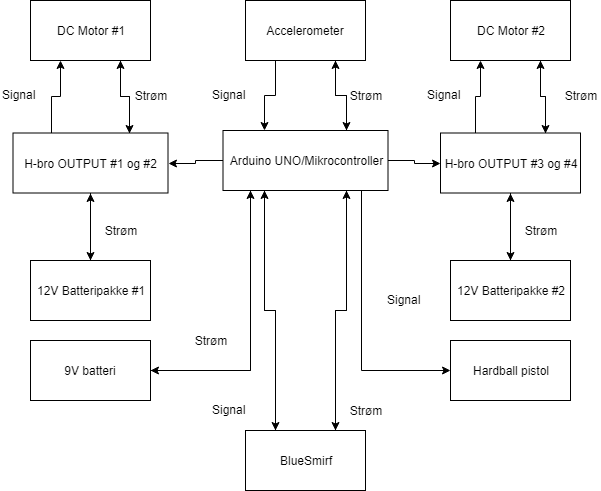
\includegraphics[scale=0.8]{Billeder/Kredsloeb1.png}
\caption{Blokdiagram af kredsløb \#1.}
\label{fig:Blokdiagram1}
\end{figure}


\begin{figure}[H]
\centering
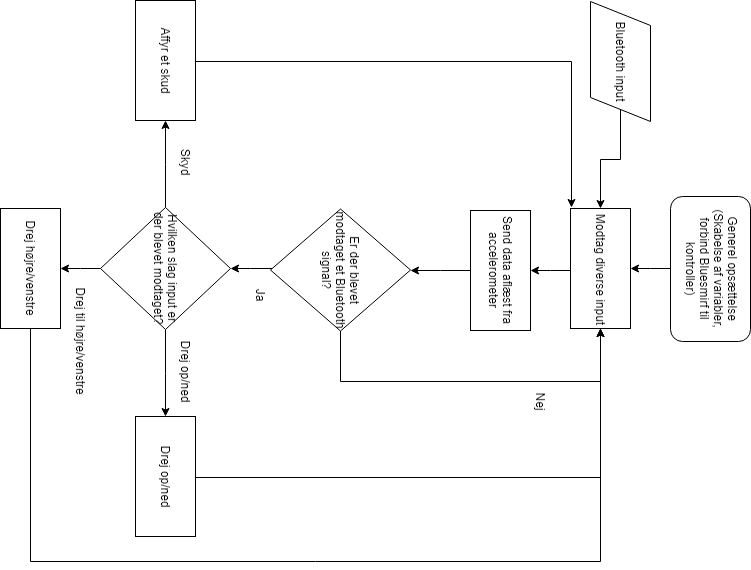
\includegraphics[scale=0.8, angle = 90]{Billeder/Flowchart1.png}
\caption{Flowdiagram af kredsløb \#1.}
\label{fig:Flowdiagram1}
\end{figure}

\newpage
\textbf{Systemdele}
\begin{itemize}
	\item Arduino UNO
\begin{itemize}
\item På blokdiagrammet (Fig. \ref{fig:Blokdiagram1}) kan det ses, at Arduinonen er forbundet til næsten alle elektroniske elementer i robotten. 
\end{itemize}

	\item 9V batteri
\begin{itemize}
\item Dette 9 volts batteri fungere som Arduinoens strømforsyning.
\end{itemize}

	\item 12V batteripakke \#1
\begin{itemize}
\item Denne batteripakke fungere som stepper motor \#1’s strømforsyning.
\end{itemize}

	\item 12V batteripakke \#2
\begin{itemize}
\item Denne batteripakke fungere som stepper motor \#2’s strømforsyning.
\end{itemize}

	\item H-bro ( LN298 ) \#1
\begin{itemize}
\item H-bro \#1 er forbundet til stepper motor \#1 og 12V batteripakke \#1. Derudover bliver H-broen kontrolleret af en Arduino, som ikke er i kredsløb med batteripakke \#1.
\end{itemize}

	\item H-bro ( LN298 ) \#2
\begin{itemize}
\item H-bro \#2 er forbundet til stepper motor \#2 og 12V batteripakke \#2. Derudover bliver H-broen kontrolleret af en Arduino, som ikke er i kredsløb med batteripakke \#2.
\end{itemize}

	\item Stepper Motor \#1
\begin{itemize}
\item Stepper \#1 er forbundet til 12V batteripakke \#1 via. H-bro \#1. Derudover er stepper motoren kontrolleret af H-bro \#1. 
\end{itemize}

	\item Stepper Motor \#2
\begin{itemize}
\item Stepper \#2 er forbundet til 12V  batteripakke \#2 via. H-bro \#2. Derudover er stepper motoren kontrolleret af H-bro \#2
\end{itemize}

	\item Accelerometer
\begin{itemize}
\item Accelerometeret er forbundet til Arduinoen, som den desuden også modtager strøm fra.
\end{itemize}

	\item Hardball pistol 
\begin{itemize}
\item Hardball pistolen indgår også i det elektriske kredsløb. Hardball pistolens skyde mekanism bliver kontrolleret af Arduinoen. I selve hardball pistolen findes der også et elektrisk kredsløb, dog er delene til dette kredsløb ikke beskrevet i blokdiagrammet, da det ikke er et selv fabrikeret elektrisk komponent. 	
\end{itemize}

\item BlueSmirf
\begin{itemize}
\item BlueSmirf modulet modtager strøm fra Arduinoen. Derudover kommunikere BlueSmirf modulet med Arduinoen.
\end{itemize}

\end{itemize}



%Kredsløb 2
\textbf{{\normalsize Kredsløb \#2}}

\begin{figure}[H]
\centering
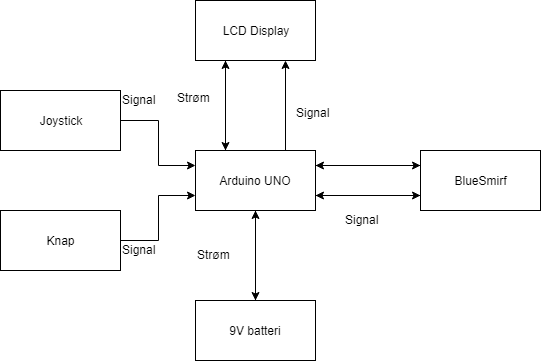
\includegraphics[scale=0.8]{Billeder/Kredsloeb2.png}
\caption{Blokdiagram af kredsløb \#2.}
\label{fig:Blokdiagram2}
\end{figure}


\begin{figure}[H]
\centering
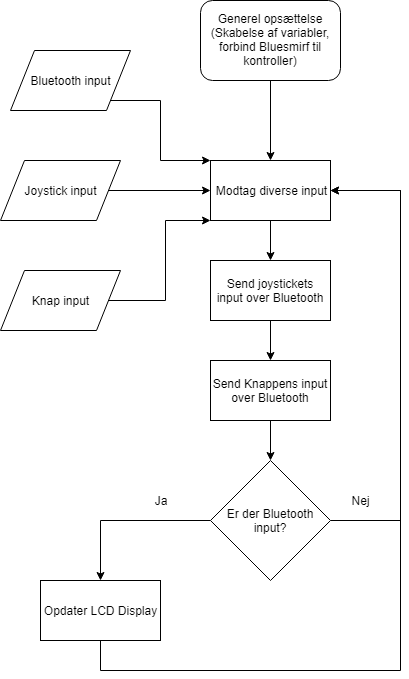
\includegraphics[scale=0.8]{Billeder/Flowchart2.png}
\caption{Flowdiagram af kredsløb \#2.}
\label{fig:Flowdiagram2}
\end{figure}

\newpage
\textbf{Systemdele}
\begin{itemize}
	\item Arduino UNO
\begin{itemize}
\item På blokdiagrammet (Fig. \ref{fig:Blokdiagram2}) kan det ses, at Arduinonen er forbundet til alle elektroniske elementer. 
\end{itemize}

	\item 9V batteri
\begin{itemize}
\item Dette 9 volts batteri fungere som Arduinoens strømforsyning.
\end{itemize}

	\item Joystick
\begin{itemize}
\item Joysticket er forbundet til Arduinoen, som måler strømmen der løber gennem joysticket.
\end{itemize}

	\item Knap
\begin{itemize}
\item Knappen er forbundet til Arduinoen, som måler strømmen der løber gennem knappen.
\end{itemize}

	\item BlueSmirf
\begin{itemize}
\item BlueSmirf modulet modtager strøm fra Arduinoen. Derudover kommunikere BlueSmirf modulet med Arduinoen.
\end{itemize}

	\item LCD Display
\begin{itemize}
\item LCD Display modulet er forbundet til Arduinoen og modtager også strøm fra Arduinoen. 
\end{itemize}

\end{itemize}







